\documentclass{article}
\usepackage[preprint]{ge2340_project}
\usepackage[utf8]{inputenc}
\usepackage[T1]{fontenc}
\usepackage{url}
\usepackage{booktabs}
\usepackage{longtable}
\usepackage{array}
\newcolumntype{L}[1]{>{\raggedright\arraybackslash}p{#1}}
\usepackage{amsmath,amssymb}
\usepackage{graphicx}
\usepackage{microtype}
\usepackage{xcolor}
\usepackage{float}
\usepackage{hyperref}
\setcitestyle{numbers,square}
\hypersetup{colorlinks=true,linkcolor=blue,citecolor=blue,urlcolor=blue,
  pdftitle={Phase 2: Course Registration Helper for Balanced Workloads},pdfauthor={}}
\urlstyle{same}
\title{Phase 2: AI Project Report\\
\large Course Registration Helper for Balanced Workloads}
\author{}


\begin{document}
\maketitle
\section{Introduction \& Problem Recap}
Students must balance prerequisites, programme requirements, interests and workload when selecting unfamiliar GE and elective courses. Our Course Registration Helper supports Computing Mathematics (CM) and Computer Science (CS) students by connecting course evidence, completed studies and a preferred stream.

Our design separates language understanding from optimisation. GPT supplies a reward policy and course-preparation hypotheses; fine-tuned Qwen expresses them as checked numerical parameters. An external optimiser selects the path while degree requirements remain fixed. The current CM experiment produces 122-credit curriculum paths and compares them with direct GPT planning. Both reach the same optimum in the three examples; our optimiser additionally verifies that maximum within its declared search space.

\section{Data Collection \& Methodology}
\textbf{Programme-specific evidence.} We assembled the handbook, CM 2025-entry path/course list, CS major/suggested-plan documents, GE information and saved Semester A/B timetables\citep{cityu-programmes}. We extract identities, credits, prerequisites, exclusions, restrictions and meetings, retaining source cohorts and years. Courses must appear in the student's designated programme document or verified GE collection. ``ONLY FOR CM'' identifies dedicated sections; compatible general sections also remain usable. Curriculum membership alone does not establish section eligibility.

Source-only mode requires compatible saved meetings. With user approval, curriculum mode can include document-listed courses as \emph{pending timetable}, without inventing dates, times or CRNs. Future A/B recurrence remains a simulation assumption.

\textbf{Model adaptation and prompts.} We adapted Qwen3-8B using rank-8 QLoRA, a frozen four-bit base and BF16 computation\citep{qwen,qlora}. The programme dataset contains 485/24/30 training/validation/test examples; the CM background update uses 244/32 plus 20 held-out checks. Relation distillation uses 149/20 examples, followed by an 82-example maximum-versus-sum correction. These evaluate familiar evidence and synthetic policies, not real workload or unseen-cohort generalisation.

Training uses system instructions, user-supplied facts/states and assistant JSON targets, with assistant-only cross-entropy loss. The current prompt permits only \texttt{reward\_parameters} and \texttt{course\_relations}. One local inference exported all eight settings and 26 links without fallback. This checks structured policy export, not independent reward quality. The latest optimiser revision did not retrain neural weights.

\textbf{Evaluation protocol.} We use fictional transcripts and controlled interventions. Both methods receive the same three histories, fixed context, six missing electives and complete reward rules. GPT uses no solver/code/browsing tools and sees no optimiser answers or scores; its final response is scored without repair. We corrected an omitted state-dependent cost before the final comparison and excluded pilot outputs. The exact comparator endpoint is unverified, so we label it GPT.

\newpage
\section{Implementation Details}
\textbf{An LLM reward model and an external planner.} Figure~\ref{fig:workflow} shows the implemented division of work. The LLM supplies utility estimates; the optimiser makes course-placement decisions. A parameter checker accepts only numerical settings and reviewed source/target/benefit links, checks finite values and bounds, and rejects schedule fields or attempts to alter hard degree requirements. The external search uses the frozen, validated packet throughout its comparisons.

\begin{figure}[H]
\centering
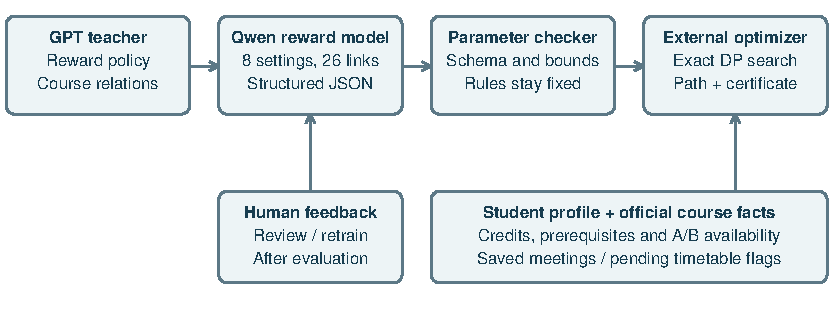
\includegraphics[width=\linewidth]{figures/workflow_reward_optimizer.pdf}
\caption{Reward-only language modelling feeds external optimisation. Human review and retraining remain a separate evaluation protocol.}
\label{fig:workflow}
\end{figure}

\textbf{GPT teaching course relations.} Our teacher authored 26 directed preparation hypotheses from saved course aims, syllabus evidence and official catalogue descriptions. Examples include MA2510 $\rightarrow$ MA3518 ($+0.30$), MA3521 $\rightarrow$ MA4529 ($+0.30$), MA3515 $\rightarrow$ EF3320 ($+0.25$), and finance GE $\rightarrow$ EF3320 ($+0.10$). They are editable content-based utility assumptions, not measured learning effects or formal prerequisites. For target $c$ and prior passed set $P(s)$,
\begin{equation}
p_c(s)=\min\!\left(0.35,\max\bigl(\{0\}\cup\{w_{ac}:a\in P(s)\}\bigr)\right).
\end{equation}
Only direct earlier passes count: there is no recursive, same-semester, self-course or repeated-course benefit. Relation checks improved from 17/20 to 20/20 before a fresh probe exposed an overlapping-benefit sum error. Corrective replay fixed that familiar probe and retained 20/20 on the unchanged held-out set.

\textbf{Human feedback after a teaching round.} A reviewer can inspect relations, parameters and generated examples after a full teacher--student training/evaluation round. Incorrect targets are corrected and mixed with source replay before retraining; held-out checks determine checkpoint retention. The project demonstrates supervised teaching and corrective replay. A formal human-annotation study remains future work, and no additional training is attributed to this report's planning experiment.

\textbf{Reward and penalty function.} For semester course set $X$, the state $s$ records earlier passes, GE areas, year, credit progress and the selected stream. We maximise
\begin{align}
U(X,s)={}&\sum_{c\in X}\bigl[g_c(s)+p_c(s)+h_c(s)+q_c(s)+z_c(s)\nonumber\\
&-\lambda_b(b_c(s)+e_c(s))-\lambda_d d_c(s)-\lambda_w w_c(s)\bigr]
+R_{\mathrm{stream}}(X,s)-O(X,s).\label{eq:utility}
\end{align}
Base value $g$, preparation $p$, core priorities $h$, prerequisite bridges $q$ and quota/timing bonuses $z$ reward progress. The student-adjustable weights $\lambda_b,\lambda_d,\lambda_w$ penalise background mismatch, difficulty and workload. These scores are configured estimates, not measured study hours. A new stream slot earns 2 points and completing one selected stream earns 6 once, multiplied by the student's stream weight.

\begin{equation}
O(X,s)=\begin{cases}
0.25[\max(0,C(X)-15)]^2,&\text{Years 1--3},\\
0.25[\max(0,C(X)-12)]^2,&\text{Year 4}.
\end{cases}\label{eq:overload}
\end{equation}
The 18-credit maximum is a separate hard constraint. A four-year recommendation must satisfy the terminal degree audit; a high reward cannot compensate for missing required credits.

\newpage
\textbf{How we solve the optimisation problem.} We use an exact finite-state dynamic programme for the remaining CM completion choices, following Bellman's principle\citep{dp}. Let $H$ be the unchanged historical transcript, $A_0$ the fixed saved course/section allocations and mandatory catch-up placements, and $M$ the unassigned electives. A state $(A,M)$ retains the complete current course-to-semester allocation. An action places course $c\in M$ in a permitted term $t$, producing $(A\cup\{(c,t)\},M\setminus\{c\})$.

For a completed allocation, our objective is
\begin{equation}
J(A)=\sum_{t=3}^{8}0.98^{t-3}U(X_t,s_t),\label{eq:pathobjective}
\end{equation}
where $s_t$ contains only earlier passes. Write $A'=A\cup\{(c,t)\}$, $M'=M\setminus\{c\}$ and let $\mathcal F$ contain terminal-feasible allocations. The recurrence is
\begin{equation}
F(A,M)=\begin{cases}
J(A),&M=\varnothing,\ A\in\mathcal F,\\
-\infty,&M=\varnothing,\ A\notin\mathcal F,\\
\max_{(c,t)\in\mathcal L(A,M)}F(A',M'),&M\ne\varnothing.
\end{cases}\label{eq:bellman}
\end{equation}
The legal-action set $\mathcal L$ enforces course membership, prior-semester prerequisites, A/B patterns, credit/course limits and exclusions. We merge identical states reached through different insertion orders. The exact mode retains every state; a resource-limit exit cannot claim a maximum. The academic discount already appears in $J$ and is not applied again to insertion steps.

\textbf{What ``maximum'' means here.} The reported experiment fixes the existing source-backed allocation and compulsory catch-up placements, then optimises six missing electives: MA4528, MA4529, MA4537, MA4546, MA4550 and MA4551. The first has two A-term choices and each other course two B-term choices, giving $2^6=64$ complete combinations before constraints. An independent Cartesian enumeration, with a different traversal order, checks all 64 combinations and reproduces the DP maximum. The resulting gap is zero \emph{within this declared completion space}; we do not claim a global optimum over every possible core-course reallocation or future catalogue.

\textbf{Graduation and evidence constraints.} The terminal audit requires at least 122 unique credits (therefore also satisfying 121), four distributional GEs covering all three areas, at least 20 elective mathematics credits outside core/capstone study, mandatory/core completion, the project/free-elective requirements and the chosen stream. At most one distributional GE is selected per semester; compulsory language/development GE is separate. Loads are flexible, with zero to six positive-credit courses and at most 18 credits per term. There is no hard five-course minimum.

CM document-listed EF/CS prerequisites are waived as the user's advisory planning assumption; mathematics prerequisites, exclusions and section restrictions remain binding. EF courses without finance-study evidence receive $e_c=1.5$, while passed/declared finance preparation removes that surcharge. Finance mismatch is 0.45 without evidence, 0.15 for introductory study and 0.05 for advanced study. These state rules apply to fixed MA3521 as well as new finance electives. EF3320 receives an additional four points in Year 4, remains legal earlier, and uses its compatible saved Semester B section when timetable evidence is attached.

For GE, a previously covered area reduces base profit from 3 to 0.3; a new area earns five extra points and GE count progress earns two while fewer than four passes are complete. In the worked paths, the credit repair is
\[
100-3\text{ (surplus GE)}+1\text{ (GE1601)}+6\text{ (project)}+18\text{ (maths)}=122.
\]
Twenty-five future credits still lack saved class details. They remain pending, with null meetings/CRNs; project parts denote one six-credit year-long course allocated three credits per term. Missing zero-credit soft-skills requirements are planned catch-up tasks requiring confirmation, not invented historical passes. A curriculum-complete result therefore remains distinct from a confirmed registration timetable.

\newpage
\section{Results \& Evaluation}
\textbf{Three matched student inputs.} Each fictional student has completed exactly 15 credits in Year 1A and 15 in Year 1B. The common Year 1A passes are MA1300, CS1302, PHY1201 and GE1401; Year 1B passes are MA1301, CHEM1200, GE1501 and GE2401. Each term also includes the profile-specific three-credit GE in Table~\ref{tab:profiles}. The fixed future course context is supplied identically to both methods within each case; it differs across cases, so this is not a causal comparison of GE histories.

\begin{table}[H]
\centering\small
\caption{Completed Year-1 GE profiles and desired stream. All listed courses are assumed passes.}
\begin{tabular}{L{0.45in}L{1.45in}L{1.45in}L{1.45in}}
\toprule
Profile & Year 1A GE & Year 1B GE & Desired stream\\\midrule
F & GE2260, Area 2 & GE1105, Area 1 & Financial Mathematics\\
N & GE1305, Area 3 & GE1113, Area 1 & Financial Mathematics\\
M & GE2134, Area 1 & GE1305, Area 3 & Enriched Mathematics\\
\bottomrule
\end{tabular}\label{tab:profiles}
\end{table}

\textbf{Actual outputs: reward model plus DP versus direct GPT.} Our method uses Qwen's validated parameter/link packet and the external DP. The baseline GPT selects placements directly from the same packet and course facts, without running the optimisation method or seeing its results. The common critic checks both outputs; it performs no repair or fallback for GPT. Table~\ref{tab:outputs} shows every elective decision, omitting clock times. Terms not listed contain the unchanged fixed course context.

{\small\setlength{\tabcolsep}{4pt}\renewcommand{\arraystretch}{1.1}
\begin{table}[H]\centering\small
\caption{Paired outputs for all six missing electives. Both methods produce the same placements in every case.}
\begin{tabular}{L{0.4in}L{2.35in}L{2.35in}}
\toprule
Profile & Qwen reward model + external DP & Direct GPT, without optimiser\\\midrule
F & Y3B: MA4529, MA4537\par Y4A: MA4528\par Y4B: MA4546, MA4550, MA4551 & Y3B: MA4529, MA4537\par Y4A: MA4528\par Y4B: MA4546, MA4550, MA4551\\\addlinespace[4pt]
N & Y3A: MA4528\par Y4B: MA4529, MA4537, MA4546, MA4550, MA4551 & Y3A: MA4528\par Y4B: MA4529, MA4537, MA4546, MA4550, MA4551\\\addlinespace[4pt]
M & Y3B: MA4537, MA4546\par Y4A: MA4528\par Y4B: MA4529, MA4550, MA4551 & Y3B: MA4537, MA4546\par Y4A: MA4528\par Y4B: MA4529, MA4550, MA4551\\\addlinespace[4pt]
\bottomrule\end{tabular}\label{tab:outputs}\end{table}}

\begin{table}[H]\centering\small
\caption{Common-checker results. Rewards are configured utility points, not measured educational outcomes.}
\begin{tabular}{lrrrrr}\toprule
Profile & DP reward & GPT reward & Gap & Credits, both & Legal / 64\\\midrule
F & 154.3121 & 154.3121 & 0.0000 & 122 & 20\\
N & 140.1263 & 140.1263 & 0.0000 & 122 & 2\\
M & 153.6550 & 153.6550 & 0.0000 & 122 & 12\\

\bottomrule\end{tabular}\label{tab:benchmark}\end{table}

Both methods pass the encoded curriculum audit in all three cases and reach the same certified completion optimum. These examples do not demonstrate a reward advantage over direct GPT. The external optimiser contributes an explicit constraint audit and a maximum certificate; GPT's response alone provides neither. This small familiar-profile benchmark does not establish superiority on unseen students, larger catalogues or a verified model endpoint. Raw final GPT answers, the corrected input packet and both scored paths are retained\citep{runs}.

\newpage
\textbf{A complete output, including fixed courses.} Table~\ref{tab:fullpath} expands profile N into its full projected path. GPT and the optimiser return the same six elective placements, so the resulting full paths are identical. The Year-1 history is unchanged, and all future grades are assumed passes for the simulation.

\begin{table}[H]\centering\small
\caption{Profile N: common full output from both methods. A star marks pending class details; zero-credit catch-up requirements are shown explicitly.}
\begin{tabular}{L{0.38in}L{3.75in}rr}\toprule
Term & Selected courses & CUs & Total\\\midrule
Y1A & MA1300, CS1302, PHY1201, GE1401, GE1305 & 15 & 15\\
Y1B & MA1301, CHEM1200, GE1501, GE2401, GE1113 & 15 & 30\\
Y2A & CS2360, CSCI1001$^{*}$ (0), GE1601$^{*}$, GE2260, MA2503, MA2508, MA2509 & 18 & 48\\
Y2B & CS2468, CSCI1002$^{*}$ (0), EF3320, MA2507, MA3511, MA3515, MA3517 & 16 & 64\\
Y3A & GE1105, MA3512, MA3525, MA4528$^{*}$, MA4545 & 15 & 79\\
Y3B & MA2510, MA3514, MA3523, MA3526, MA3530 & 13 & 92\\
Y4A & MA3518, MA3521, MA4530 (A)$^{*}$, MA4542 & 12 & 104\\
Y4B & MA4529$^{*}$, MA4530 (B)$^{*}$, MA4537$^{*}$, MA4546$^{*}$, MA4550$^{*}$, MA4551$^{*}$ & 18 & 122\\

\bottomrule\end{tabular}\label{tab:fullpath}\end{table}

All three repaired paths contain four distributional GE passes across Areas 1--3, 30 elective mathematics credits, 45 core credits and six project credits, with the selected stream complete under the encoded rules. Profile N's advanced B-term electives follow MA2510 in Year 3B and MA3518/MA3521 in Year 4A. Its 18-credit final term therefore incurs the configured nine-point Year-4 overload penalty. A 12- or 13-credit term remains valid because the whole path now reaches 122; we do not force five courses in every term.

\textbf{Parameter sensitivity changes a tool decision.} Holding profile F and its course links fixed, changing only the Year-4 overload coefficient changes the optimal placement (Table~\ref{tab:sensitivity}). This verifies that the optimiser responds to supplied parameters rather than reproducing a fixed language-model answer. The zero-weight run is a counterfactual test; the configured policy remains 0.25.

\begin{table}[H]\centering\small
\caption{Controlled overload intervention, with 122 credits retained.}
\begin{tabular}{lrrr}\toprule
Year-4 coefficient & Year 3B CUs & Year 4B CUs & Total\\\midrule
0.25, configured & 18 & 15 & 122\\
0, counterfactual & 15 & 18 & 122\\\bottomrule
\end{tabular}\label{tab:sensitivity}\end{table}

\textbf{Dependency experiment: how earlier study changes rewards.} Our earlier 12 paired interventions hold year, base profit, score vector and penalty weights fixed while excluding credit-progress and overload effects. All match their predeclared policy effects. Table~\ref{tab:dependency} retains representative relations; they are computational tests of configured mechanisms.

\begin{table}[H]\centering\small
\caption{Representative dependency effects, with other tested components fixed.}
\begin{tabular}{L{2.5in}L{0.75in}L{1.7in}}\toprule
Changed history or preference & Target & Reward effect\\\midrule
Pass MA2508 & MA3515 & Preparation $+0.20$\\
Pass MA2509 & GE2134 & Preparation $+0.15$\\
Covered Area 1 replaces Area 2 & GE1113 & Base reward $-2.70$\\
Pass GE2260; finance selected & MA3521 & Stream reward $+4.00$\\
Pass MA2503; portfolio mathematics & EF3320 & Preparation $+0.20$\\\bottomrule
\end{tabular}\label{tab:dependency}\end{table}

\newpage
\section{Discussion}
Our contribution separates interpretable preferences from auditable optimisation. Students specify a stream and three penalty weights; earlier passes change preparation, background and stream rewards. Qwen supplies checked rewards while the external engine selects and explains the route. Preference changes need no retraining. Software verification now covers 111 checks, including parameter rejection, the 122-credit boundary, relation aggregation, independent enumeration and the comparison critic.

\textbf{What the comparison supports.} GPT matches all three maxima, supporting a verification benefit rather than better recommendations here. The task is small, profiles are familiar and fixed contexts differ across cases. The certificate covers the remaining electives, with source-backed and catch-up placements fixed. Core rescheduling, different elective pools or complete section choices require a new search and broader certificate. A resource-limit exit makes no maximum claim.

\textbf{What failed and remains uncertain.} The source-only simulation exhausted a 100-credit pool and displayed an incomplete diagnostic, including an empty Year 4B. We corrected the recommendation boundary and introduced authorised curriculum mode. It reaches 122 while keeping 25 future credits pending. Overdue zero-credit catch-up arrangements also need confirmation. A curriculum audit cannot establish seats, clash-free registration or official graduation approval.

An omitted state-dependent cost can distort a comparison despite identical course lists. We corrected the fixed MA3521 finance-mismatch rule for both methods and excluded the pilot answers, retaining the error record. The comparator's unverified endpoint also limits model-specific conclusions.

The graph contains content-based hypotheses, not measured hours or causal effects. Correct policy export does not show independent reward learning. Human review should assess relations and workload estimates before further retraining. Consented student outcomes, cohort-consistent rules and confirmed sections are needed to test workload balance and generalisation. Real-transcript studies require consent and minimal retention.

\section{Conclusion}
Our helper uses an LLM for rewards and relations, and external dynamic programming for path selection. The three CM examples reach 122 credits and the certified completion maximum; direct GPT matches every output. The demonstrated benefits are constraint enforcement, parameter sensitivity and a verifiable maximum, with pending timetables visible. Next we will expand the search space and validate rewards against reviewed workload and student outcomes.

\begin{thebibliography}{9}
\footnotesize\setlength{\itemsep}{0pt}\setlength{\parsep}{0pt}
\bibitem[Yang et~al.(2025)]{qwen}
A. Yang et al., ``Qwen3 Technical Report,'' arXiv:2505.09388, 2025. \url{https://arxiv.org/abs/2505.09388}.
\bibitem[Dettmers et~al.(2023)]{qlora}
T. Dettmers et al., ``QLoRA: Efficient Finetuning of Quantized LLMs,'' 2023. \url{https://arxiv.org/abs/2305.14314}.
\bibitem[Tedrake()]{dp}
R. Tedrake, ``Dynamic Programming,'' \emph{Underactuated Robotics}, MIT. \url{https://underactuated.mit.edu/dp.html}.
\bibitem[CityUHK(2022--2026)]{cityu-programmes}
CityUHK, supplied Student Handbook 2026--27, CM 2025-entry normative path and designated course list, CS major/suggested-plan documents, GE and saved Semester A/B timetables. Current advanced-course rules: \url{https://www.cityu.edu.hk/catalogue/ug/current/course/MA4537.htm} and corresponding course-code pages.
\bibitem[Project experiment records(2026)]{runs}
Project experiment records, 21--24 November 2026: reward-only Qwen export, three exact completion runs, independent 64-assignment checks, controlled parameter interventions and the corrected blind direct-GPT comparison. Raw inputs/outputs and hashes accompany this report.
\end{thebibliography}
\end{document}
